
\chapter{Methodology}

The process of data collection began with analysis of the physical principles underlying optical light emission. For illustration purposes, see \ref{fig:secondFig}.

\section{The Various Types of Light}

Depending on the energy of a photon, it may be referred to as ``light'' (in the case of optical photons) or as something else -- for example, a gamma ray. By convention, there are many names for these particles.

\subsection{Low-energy photons}

The lowest energy electromagnetic radiation is carried by radio waves.

\subsection{Intermediate-energy photons}

These include several types of radiation, including the usually-harmful \gls{uv}.

\subsubsection{Microwaves}

Microwaves have wavelengths on the order of \SI{1e-2}{\meter}, or a few \si{\centi\meter}.

\subsubsection{Visible light}

Visible light is that which is detectable by the human eye, with wavelengths about \SIrange{380}{750}{\nano\meter}.

\begin{rotatepage}
\begin{sidewaysfigure}[!t]
    \centering
    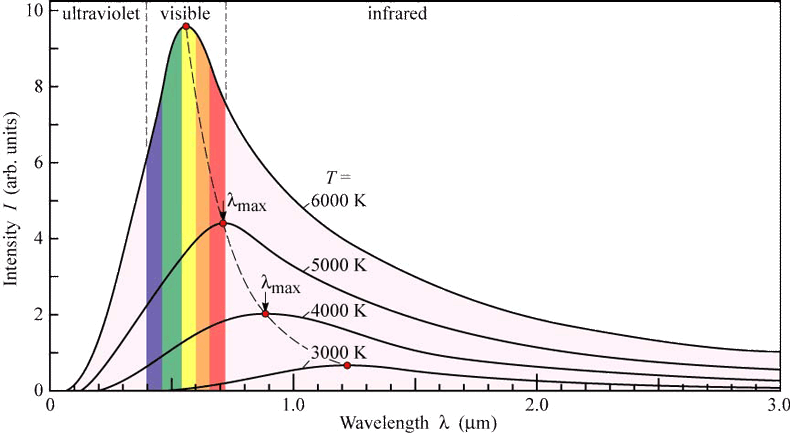
\includegraphics[width=\textwidth]{graphics/sampleFig2.png}
    \caption[Black-body radiation]{Spectra of black-body radiation at various temperatures, according to Wien's displacement law \cite{wannier1987statistical}.}
    \label{fig:secondFig}
\end{sidewaysfigure}
\end{rotatepage}
